%%
%% This is file `sample-authordraft.tex',
%% generated with the docstrip utility.
%%
%% The original source files were:
%%
%% samples.dtx  (with options: `authordraft')
%% 
%% IMPORTANT NOTICE:
%% 
%% For the copyright see the source file.
%% 
%% Any modified versions of this file must be renamed
%% with new filenames distinct from sample-authordraft.tex.
%% 
%% For distribution of the original source see the terms
%% for copying and modification in the file samples.dtx.
%% 
%% This generated file may be distributed as long as the
%% original source files, as listed above, are part of the
%% same distribution. (The sources need not necessarily be
%% in the same archive or directory.)
%%
%% The first command in your LaTeX source must be the \documentclass command.
\documentclass[sigconf]{acmart}
%% NOTE that a single column version may required for 
%% submission and peer review. This can be done by changing
%% the \doucmentclass[...]{acmart} in this template to 
%% \documentclass[manuscript,screen]{acmart}
%% 
%% To ensure 100% compatibility, please check the white list of
%% approved LaTeX packages to be used with the Master Article Template at
%% https://www.acm.org/publications/taps/whitelist-of-latex-packages 
%% before creating your document. The white list page provides 
%% information on how to submit additional LaTeX packages for 
%% review and adoption.
%% Fonts used in the template cannot be substituted; margin 
%% adjustments are not allowed.

%%
%% \BibTeX command to typeset BibTeX logo in the docs
\AtBeginDocument{%
  \providecommand\BibTeX{{%
    \normalfont B\kern-0.5em{\scshape i\kern-0.25em b}\kern-0.8em\TeX}}}

%% Rights management information.  This information is sent to you
%% when you complete the rights form.  These commands have SAMPLE
%% values in them; it is your responsibility as an author to replace
%% the commands and values with those provided to you when you
%% complete the rights form.
%\setcopyright{acmcopyright}
%\copyrightyear{2021}
%\acmYear{2021}
%\acmDOI{10.1145/1122445.1122456}

%% These commands are for a PROCEEDINGS abstract or paper.
%\acmConference[CS573 Fall '21]{CS573 Fall '21: Data Mining}{August 23--December 08, 2021}{Purdue University, IN}
%\acmBooktitle{CS573 Fall '21: Final Project Proposal,
%  September 26, 2021, Purdue University, IN}
%\acmPrice{15.00}
%\acmISBN{978-1-4503-XXXX-X/18/06}


%%
%% Submission ID.
%% Use this when submitting an article to a sponsored event. You'll
%% receive a unique submission ID from the organizers
%% of the event, and this ID should be used as the parameter to this command.
%%\acmSubmissionID{123-A56-BU3}

%%
%% The majority of ACM publications use numbered citations and
%% references.  The command \citestyle{authoryear} switches to the
%% "author year" style.
%%
%% If you are preparing content for an event
%% sponsored by ACM SIGGRAPH, you must use the "author year" style of
%% citations and references.
%% Uncommenting
%% the next command will enable that style.
%%\citestyle{acmauthoryear}

%%
%% end of the preamble, start of the body of the document source.
\begin{document}

%%
%% The "title" command has an optional parameter,
%% allowing the author to define a "short title" to be used in page headers.
\title{%
  Midterm Report \\
  \large CS 573 - Data Mining - Fall 2021}

%%
%% The "author" command and its associated commands are used to define
%% the authors and their affiliations.
%% Of note is the shared affiliation of the first two authors, and the
%% "authornote" and "authornotemark" commands
%% used to denote shared contribution to the research.
\author{Reece Jones}
\affiliation{%
    \institution{Purdue University}
    \country{United States}}
\email{jone1926@purdue.edu}

\author{Eli Silkov}
\affiliation{%
    \institution{Purdue University}
    \country{United States}}
\email{esilkov@purdue.edu}

\author{Nathan Merz}
\affiliation{%
    \institution{Purdue University}
    \country{United States}}
\email{merzn@purdue.edu}

\author{Patrick Li}
\affiliation{%
    \institution{Purdue University}
    \country{United States}}
\email{li3992@purdue.edu}

\author{Varun Vora}
\affiliation{%
    \institution{Purdue University}
    \country{United States}}
\email{vora18@purdue.edu}

%%
%% By default, the full list of authors will be used in the page
%% headers. Often, this list is too long, and will overlap
%% other information printed in the page headers. This command allows
%% the author to define a more concise list
%% of authors' names for this purpose.
\renewcommand{\shortauthors}{Jones, Silkov, Merz, Li, Vora}

%%
%% The abstract is a short summary of the work to be presented in the
%% article.
\begin{abstract}
In this article we discuss what we have learned during the literature review process, and how we plan to apply what we have learned to the modeling and practical application tasks. We then discuss the results of our data analysis, followed by the preliminary results of our modeling efforts. We conclude with the challenges that we have faced, how we have overcome them, and what remaining tasks we plan to complete.
\end{abstract}

%%
%% The code below is generated by the tool at http://dl.acm.org/ccs.cfm.
%% Please copy and paste the code instead of the example below.
%%
\begin{CCSXML}
<ccs2012>
   <concept>
       <concept_id>10010147.10010257</concept_id>
       <concept_desc>Computing methodologies~Machine learning</concept_desc>
       <concept_significance>500</concept_significance>
       </concept>
 </ccs2012>
\end{CCSXML}

\ccsdesc[500]{Computing methodologies~Machine learning}

%%
%% Keywords. The author(s) should pick words that accurately describe
%% the work being presented. Separate the keywords with commas.
\keywords{datasets, CS573, food, recipes, machine learning, analysis, visualization, project, group}

%%
%% This command processes the author and affiliation and title
%% information and builds the first part of the formatted document.
\maketitle

\section{Literature Review}
\subsection{Recommendation Systems}
Insinkaye et al. \cite{RSSurvey} provide a survey of the field of recommendation systems. The authors discuss the properties, construction, benefits, and downsides of using collaborative and content-based filtering for recommendation systems.

Collaborative filtering looks for patterns between users to generate recommendations. These patterns can be extracted through the use of memory-based methods like K-Nearest Neighbors, or can be extracted through the use of data mining techniques and machine learning models like clustering and neural networks. Collaborative filtering is powerful, because it requires little prior domain-specific knowledge, and is capable of making cross-category recommendations on the basis of user similarity. However, collaborative filtering requires a significant amount of user-data to be effectively trained \cite{RSSurvey}.

In contrast, content-based filtering looks for patterns between individual items to generate recommendations. This process requires items to be meticulously and consistently annotated for accurate recommendations. Additionally, content-based filtering requires domain specific knowledge as the content must be intrinsically analyzed, which often means a significant amount of pre-processing and feature engineering are required before successful models can be learned and applied within content-based filtering systems \cite{RSSurvey}.

Additionally, ensembles of collaborative and content-based filtering techniques can be created to build hybrid filtering techniques. This method seeks a balance between the two methodologies, where both similar items and items the user likely wants are both recommended. Depending on the specific type of recommendation system that is desired, multiple different types of hybrid filtering techniques can be used. However, hybrid filtering requires more effort than either content-based or collaborative filtering as not only must both systems must be developed, but their recommendations must also be merged and ranked together according to the hybrid filtering technique \cite{RSSurvey}.

The article gives a good overview of how different recommendation systems can be constructed and the trade offs inherent in certain systems. These recommendation system techniques can be used in some of our models and applications.

Ueta et al. \cite{RSRecipe} demonstrate a recipe recommendation system based on user submitted queries. The authors describe a system where a co-occurrence dictionary is used to map relationships between nouns and nutrients. These related nutrients are then used as search parameters for recipes.

The co-occurrence dictionary can be expanded to our use case to encode relationships between ingredients, metadata, and recipes. These relationships can either be used within our models, or as a part of our novel recipe generator.

\subsection{Natural Language Processing}
\begin{figure}[h]
  \centering
  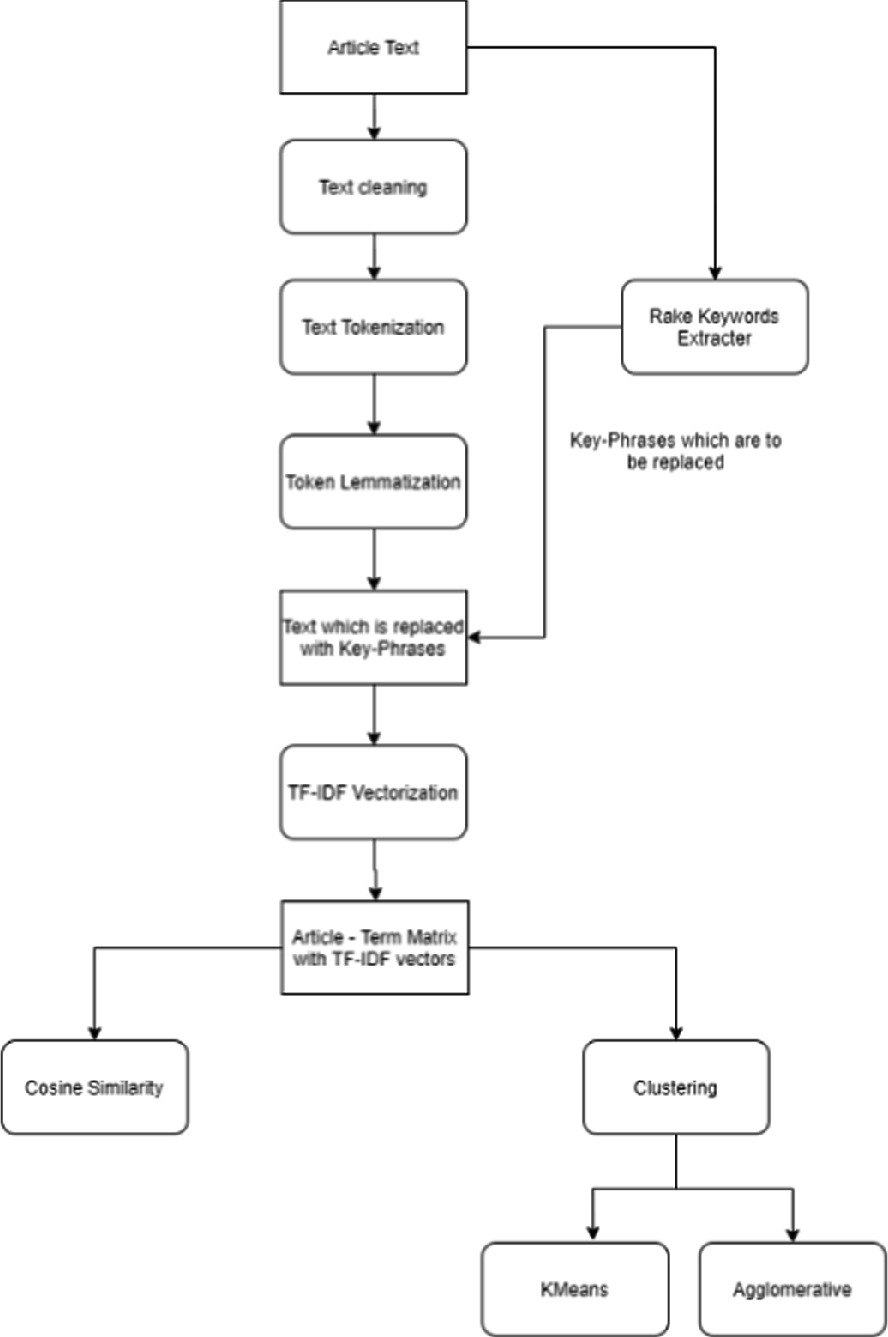
\includegraphics[width=\linewidth]{article-rs}
  \caption{Functional Diagram of Unsupervised Content-Based Article Recommendation System \cite{RSArticle}}
  \Description{A block diagram with arrows pointing between pre-processing and processing steps}
\end{figure}
Renuka et al. \cite{RSArticle} demonstrate an unsupervised content-based approach towards a recommendation system that incorporates natural language processing. The devised system pre-processes articles to build a term matrix of TF-IDF values. This term matrix is then passed to either a cosine similarity content-based filtering model or to content-based clustering models to find similar articles. The functional diagram can be seen in Figure 1.

Input articles were pre-processed by cleaning the text of any non-alphabetic characters, tokenizing by spaces, lemmatizing with the nltk python package, extracting keywords using rapid automatic keyword extraction (RAKE), individual converting tokens into n-grams based on the phrases extracted by RAKE, removing stopwords which do not contribute to the meaning of the article, then finally converting the remaining term-matrix into a TF-IDF term matrix. The dimensionality of the data is then reduced using latent semantic analysis, which performs better than principle component analysis with sparse data. This dimensionality reduction is important to reduce the sparsity of the dataset, remove redundant information, and ultimately improve model performance \cite{RSArticle}.

Two primary approaches are used in the article: cosine similarity, and clustering. In the first approach, cosine similarity is applied to find articles similar to articles the user has not read. While this method is simple and effectively applied on a TF-IDF term matrix, it fails to capture the complexity of additional features, because all features are uniformly weighted under cosine similarity \cite{RSArticle}.

The second approach uses clustering to find similar articles based on the similarity between their word groupings. Two clustering methods are discussed in the article: K-Means and Agglomerative clustering. K-Means performs similarly to the cosine similarity-based approach, being okay at recommending generic articles and good at recommending articles under a specific topic. Agglomerative clustering likewise also performed good at recommendations for a specific topic, but failed at general recommendations \cite{RSArticle}.

The authors conclude that the cosine similarity model performed best, with K-Means coming in second, and Agglomerative coming in last \cite{RSArticle}.

Ultimately, Renuka et al. show how simple natural language processing techniques can be applied with high success to recommendation systems. These efforts can be further improved by introducing additional features to the TF-IDF term matrix, and other content-based models like support vector machines or neural networks.

Jermsurawong et al. \cite{NLPSIMMR} introduces Simplified Ingredient Merging Map in Recipes (SIMMR), a recipe representation structure that encodes recipes as dependency trees of both ingredients and instructions. SIMMR builds on the Minimal Instruction Language for the Kitchen (MILK) by simplifying the modeling assumptions. Lastly, the authors introduce their SIMMR parser which takes text as input and outputs SIMMR structures.

Each internal node in the SIMMR dependency tree is either an ingredient or an instruction, and each leaf node must be an ingredient. Each connecting edge between nodes represents a dependency relationship. In effect, this means that any node requires all connected nodes below itself to be satisfied before action can be taken on the present node. Additionally, instruction nodes can only output a single ingredient. This is a simplification made from MILK, and is done, because only about 3\% of recipes have instructions where two ingredients are output, many of which discard the second output \cite{NLPSIMMR}.

The SIMMR parser consists of two phases: the first phase in which ingredients are linked to instructions, and the second phase in which instructions are linked to other instructions. Ingredients and instructions are processed like usual: remove stop words, remove quantities, tokenization, etc.. The primary focus is instead placed on how ingredients and instructions are linked together. To do this, the authors trained classification models to predict whether an ingredient and instruction or instruction and instruction had a link between one another. As a result two models were trained, one for each case \cite{NLPSIMMR}.

For the linkage classification models, an SVMRank classification model was used for both. Additionally, a significant number of features like the number of unigram matches, degree of similarity measures, and binary term vectors are computed to improve model performance \cite{NLPSIMMR}.

Ultimately, SIMMR shows an impressive 93.5\% accuracy for full SIMMR tree construction \cite{NLPSIMMR}. This shows that SIMMR can serve as a strong representation stucture of arbitrary recipes. Because of this strong representation, SIMMR will be extremely useful for generative tasks and transforming recipe text for the purpose of featurization during modeling.

\subsection{Recipe Modeling}
%% Reece: GPT-2 is freely available, so we may be able to recreate the model in the paper. Not sure how time consuming that would be though... If we do, we should also incorporate the metadata that is in the dataset to make better predictions.
%% Reece: https://recipegpt.org/
Lee et al. \cite{NLPRecipeGPT} demonstrate recipe generation models using a pre-trained and fine-tuned GPT-2 model that are capable of producing convincing recipes. The article discusses the pre-processing steps, and methodologies used to train the model.

The recipes are pre-processing by removing numerals, quantity words, comments, and other rule-based filtering. The recipes are further filtered by removing recipes containing non-ingredients and non-instructions. Tokens are then added to the beginning and end of recipe sections, and the sections are then shuffled according to the desired generation target. Lastly, byte-pair encoding is used to applied so that the model can be learned with GPT-2 \cite{NLPRecipeGPT}.

The learned models produce convincing results with strong evaluation metric scores, despite the learning process taking 5 days to converge \cite{NLPRecipeGPT}. This article will serve is a reference for ideas we can use for pre-processing, model learning, and evaluation metrics.

Reusch et al. \cite{NLPRecipeGM} demonstrate an alternative approach to generating recipes that can sometimes outperform RecipeGPT. The authors propose the use of a hierarchical sequence-to-sequence neural network model to generate both instruction and recipe title text. Reusch et al. also call for the use of new metrics for recipe language generation, as existing metrics do not successfully cover the creative and diverse aspects of recipes.

Ultimately, RecipeGM is successful at producing convincing results, with strong text variety, and trades blows with RecipeGPT, despite RecipeGPT using GPT-2, which the authors recognize as a stronger architecture for text-generation tasks \cite{NLPRecipeGM}. This article is useful, because it further reinforces natural language methodologies, provides additional evaluation metrics, and shows the importance of small changes.

\subsection{Conclusion}
The recommendation system principles and examples discussed will serve as a baseline for the implementation of some of our models and practical applications. Further improvements can be made on the article recommendation system introduced by Renuka et al. \cite{RSArticle} by introducing additional features, introducing more complex models, and using a hybrid filtering technique. The concept of the co-occurrence dictionary used by Ueta et al \cite{RSRecipe} can also be used to model relationships between ingredients, and thus used in our modeling. The SIMMR parser discussed by Jermsurawong et al \cite{NLPSIMMR} can be used for creating features during the modeling phase and potentially used in the practical application. Lastly, RecipeGPT \cite{NLPRecipeGPT} and RecipeGM \cite{NLPRecipeGM} serve as examples for the complex text-generation modeling tasks. The approaches used by both articles can be merged together and applied with other methodologies collected during the literature review to build a powerful text-generation model. However, exact use of the methods shown in these works may be impractical, because of high model training times.

\section{Preliminary Results}
\subsection{Data Analysis}
The majority of recipes have a preparation time that is less than 1 hour, with a mean preparation time of 80 minutes Most recipes are completed in under 20 steps. The distribution of recipe steps is skewed right.

\begin{figure}[h]
  \centering
  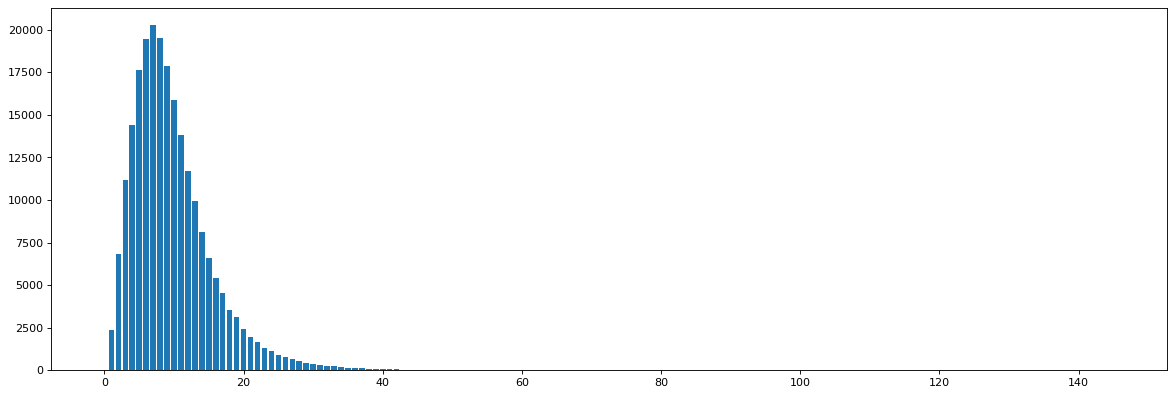
\includegraphics[width=\linewidth]{steps.png}
  \caption{Distribution of recipes by number of steps}
\end{figure}

A small group of ingredients appear in a large number of recipes. The top 100 ingredients represent 33 percent of ingredient frequency (sum of the count for the top 100 ingredients across all recipes divided by the sum of the total ingredient count for all recipes). The top 3 ingredients (salt, low fat butter and durkee onions) are present in 29 percent, 29 percent and 17 percent of recipes. The authors also explored the frequency of words in recipe names. Here, we see a similar trend to ingredients, where the top 100 words represent 49 percent of the cumulative word count. Going forward, we plan to tokenize recipe names in order to isolate the subject/most important word in the title.

Next, we examined temporal trends in the recipe data. Protein and carbs have been gaining share of the average recipe's macro breakdown from 2016 to 2018. However, these numbers have remained consistent over the last 20 years. 

\begin{figure}[h]
  \centering
  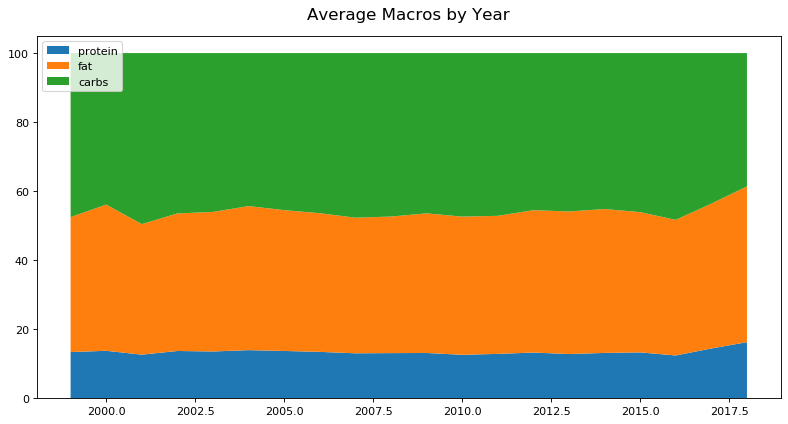
\includegraphics[width=\linewidth]{macros.png}
  \caption{Change in macro shares over time}
\end{figure}

Interestingly, the average preparation time and average number of steps have also increased in the 2016 - 2018 period, after remaining fairly over the 10 year period before that. 

\begin{figure}[h]
  \centering
  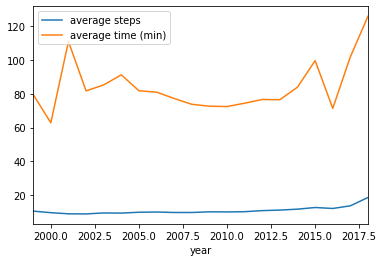
\includegraphics[width=\linewidth]{steps time over time.png}
  \caption{Historical average preparation time and number of steps}
\end{figure}

The strongest correlations observed in the dataset are correlations between macro proportions, which is expected considering that the proportions must sum to 1. The next strongest correlation is between the number of steps and the preparation time, which is to be expected as well. There are no other significant correlations between ordinal variables. 

\begin{figure}[h]
  \centering
  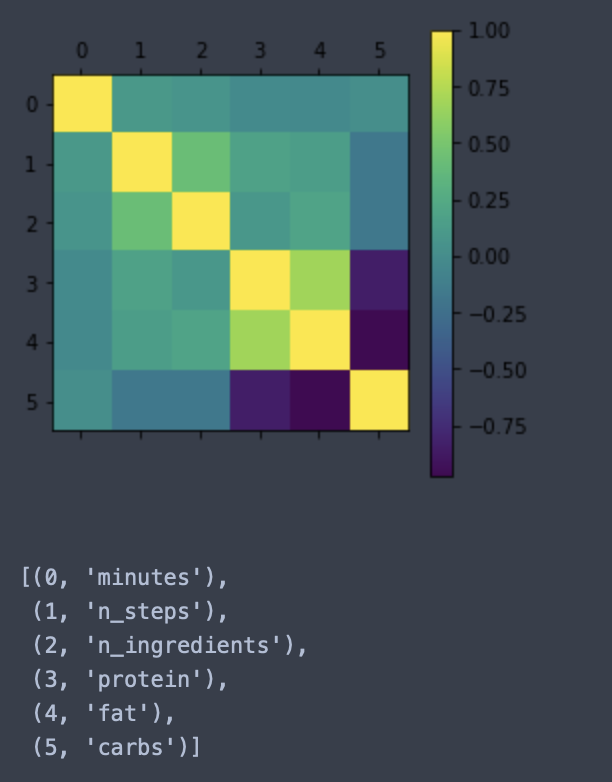
\includegraphics[width=\linewidth]{corrplot.png}
  \caption{Correlation matrix for RAW\_recipes dataset}
\end{figure}

\subsection{Models}
Initial modeling efforts focused on number of ingredients and cooking time. One fifth of the data was withheld as a test dataset for final evaluation. Training data was split again into train (114090 entries) and validation (28522 entries) sets. Both modeling efforts use the LightGBM library. For preprocessing, outliers outside the 5-th and 95-th percentiles are capped at the respective percentile. Cooking times are grouped into to 25 bins. Prediction and evaluation was done using the following columns: 'ingredient\_0', 'ingredient\_1', 'ingredient\_2', 'ingredient\_3', 'ingredient\_4', 'calorie\_level', 'num\_ingredients', 'minutes', 'n\_steps'. The column being predicted was withheld from the training data for that prediction. LightGBM training uses the following parameters (we plan to use cross-validation to fine tune parameters before the final report):  

\begin{verbatim}
"objective": "multiclass",
"lambda_l2": .05,
"min_data_in_leaf": 100,
"is_unbalance": True,
"metric": "multi_logloss",
"boost_from_average": False
\end{verbatim}

Intermediate evaluation is performed on our validation set. Performance is significantly better than predicting the most common value, however it still has overall low accuracy. The number of ingredients can be predicted with an accuracy of 23.133 \%; the most common ingredient bin, 8, accounts for 12.299 \% of validation data. The cooking time range can be predicted with an accuracy of 27.165 \%; the common common range accounts for 17.467 \% of validation data. Next steps include adding cross-validation parameter tuning and examining other model types.


\section{Challenges}

As we proceeded through our literature review, we realized that our initial dataset \cite{FoodComRecipe} of about 178,267 recipes was of insufficient size to train text-generation models on. Thus, we have elected to adopt a second dataset for text-generation tasks: Recipe1M+ \cite{Recipe1M}. This dataset contains approximately one million recipes, complete with ingredients, steps, and images. This new dataset should be sufficient for the complex text-generation modelling tasks.

\section{Conclusion}
Thus far we have completed the literature review and data analysis, and have begun our modeling efforts. Moving forward, our focus will be on completing the modeling tasks, and subsequently incorporating the learned models into our practical applications.

%
%%
%% The acknowledgments section is defined using the "acks" environment
%% (and NOT an unnumbered section). This ensures the proper
%% identification of the section in the article metadata, and the
%% consistent spelling of the heading.
\begin{acks}
\end{acks}

%%
%% The next two lines define the bibliography style to be used, and
%% the bibliography file.
\bibliographystyle{ACM-Reference-Format}
\bibliography{midterm-refs}
%% Shuyang Li, “Food.com Recipes and Interactions.” Kaggle, 2019, doi: 10.34740/KAGGLE/DSV/783630.
%%
%% If your work has an appendix, this is the place to put it.
%\appendix

\end{document}
\endinput
%%
%% End of file `sample-authordraft.tex'.
